\documentclass[a4paper,12pt]{article} % тип документа

% Поля страниц
\usepackage[left=2.5cm,right=2.5cm,
    top=2cm,bottom=2cm,bindingoffset=0cm]{geometry}
    
%Пакет дял таблиц   
\usepackage{multirow} 
    
%Отступ после заголовка    
\usepackage{indentfirst}

% Рисунки
\usepackage{floatrow,graphicx,calc}
\usepackage{wrapfig}

%%% Работа с картинками
\usepackage{graphicx}  % Для вставки рисунков
\graphicspath{{images/}}  % папки с картинками
\setlength\fboxsep{3pt} % Отступ рамки \fbox{} от рисунка
\setlength\fboxrule{1pt} % Толщина линий рамки \fbox{}
\usepackage{wrapfig} % Обтекание рисунков и таблиц текстом

% Работа со списками
\renewcommand{\labelitemi}{\textendash}

\usepackage{enumitem}
\setlist[enumerate]{leftmargin=10pt, itemsep=2pt, topsep=2pt}

% Создаём новый разделитель
\DeclareFloatSeparators{mysep}{\hspace{1cm}}

% Ссылки?
\usepackage{hyperref}
\usepackage[rgb]{xcolor}
\hypersetup{				% Гиперссылки
    colorlinks=true,       	% false: ссылки в рамках
	urlcolor=blue          % на URL
}

%  Русский язык
\usepackage[T2A]{fontenc}			% кодировка
\usepackage[utf8]{inputenc}			% кодировка исходного текста
\usepackage[english,russian]{babel}	% локализация и переносы

% Математика
\usepackage{amsmath,amsfonts,amssymb,amsthm,mathtools}

%%% Дополнительная работа с математикой
\usepackage{amsmath,amsfonts,amssymb,amsthm,mathtools} % AMS
\usepackage{icomma} % "Умная" запятая: $0,2$ --- число, $0, 2$ --- перечисление

% Что-то 
\usepackage{wasysym}


\begin{document}
\begin{center}
	\footnotesize{ФЕДЕРАЛЬНОЕ ГОСУДАРСТВЕННОЕ АВТОНОМНОЕ ОБРАЗОВАТЕЛЬНОЕ 			УЧРЕЖДЕНИЕ ВЫСШЕГО ОБРАЗОВАНИЯ}\\
	\footnotesize{МОСКОВСКИЙ ФИЗИКО-ТЕХНИЧЕСКИЙ ИНСТИТУТ\\(НАЦИОНАЛЬНЫЙ 			ИССЛЕДОВАТЕЛЬСКИЙ УНИВЕРСИТЕТ)}\\
	\footnotesize{ФИЗТЕХ-ШКОЛА ФИЗИКИ И ИССЛЕДОВАНИЙ им. ЛАНДАУ\\}
	\hfill \break
	\hfill \break
	\hfill \break
	\hfill \break
\end{center}

\begin{center}   
    \hfill \break
	\hfill \break
	\hfill \break
	\hfill \break    \hfill \break
	\hfill \break
	\hfill \break
	\hfill \break
    \hfill \break
    \hfill \break
	\hfill \break
	\large{Лабораторная работа № 2.3.1 \\\textbf{Получение и измерение вакуума}}\\
	\begin{flushright}
		Плотникова Анастасия Александровна\\
		Группа Б02-406
	\end{flushright}
	\hfill \break
	\hfill \break
	\hfill \break
\end{center}
\hfill \break
\hfill \break
\hfill \break
\hfill \break
\hfill \break
\hfill \break
\hfill \break
\hfill \break
\hfill \break
\hfill \break
\hfill \break
\hfill \break
\hfill \break
\begin{center}
	Долгопрудный, 2025 г.
\end{center}
\thispagestyle{empty}
\newpage
	\textbf{Цель работы:}\\ 
  1) измерение объёмов форвакуумной и высоковакуумной частей установки; \\
  2) определение скорости откачки системы в стационарном режиме, а также по ухудшению и по улучшению вакуума.
	\hfill \break
	
	\textbf{В работе используются:}\\ 
  вакуумная установка с манометрами: масляным, термопарным и ионизационным.
	
\section*{Теоретическая справка}

\textbf{Def.} Число Кнудсена — отношение длины свободного пробега $\lambda$ к характерному размеру. Отвечает за критерии применимости законов диффузии, вязкости и теплопроводности.

\begin{equation}
  \text{Kn} = \frac{\lambda}{d}
\end{equation}
$\text{Kn} \ll 1$ — низкий вакуум \\
$\text{Kn} \sim 1$ — средний вакуум \\
$\text{Kn} \gg 1$ — высокий вакуум 

\smallskip

\noindent В обычных лабораторных установках ($d \approx 10$ см): \\
$P > 10^2$ Па (1 торр) — низкий вакуум \\
$10^{-1} < P < 10^2$ Па ($10^{-3}-1$ торр)— средний вакуум \\
$P < 10^{-1}$ Па ($10^{-3}$ торр) — высокий вакуум 

\subsection*{Течение разреженного газа по трубе}

Будет считать газ разреженным настолько, что его молекулы на всех длине трубы $(L, r)$ не сталкиваются между собой и соударяются только со стенкам трубы.

Диаметр трубы $2r$ — среднее расстояние, которое молекула  проходит без соударений. Аналог длины свободного пробега.

Рассмотрим течение разреженного газа через трубу как процесс диффузии с длиной свободного пробега $\lambda = 2r$. 

\begin{equation}
  \label{dN_dt}
  \frac{dN}{dt} = D \frac{dn}{dx} S,
\end{equation}
где $S = \pi r^2$, $D$ — коэффициент диффузии.

\begin{figure}
  \centering
  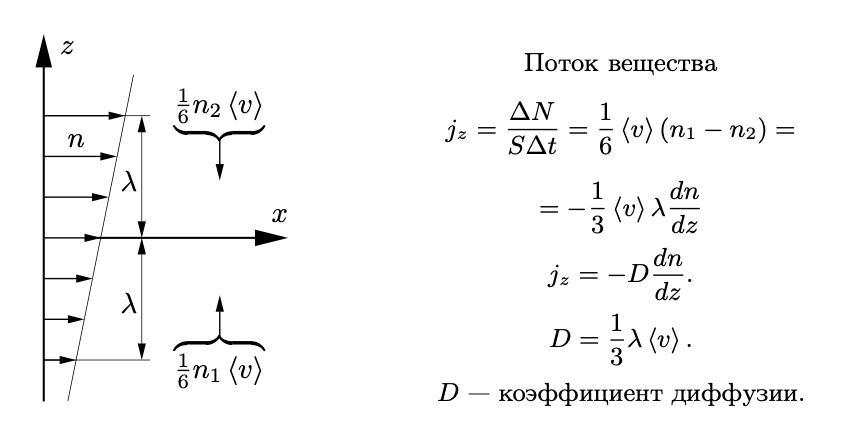
\includegraphics[scale = 0.75]{images/eq.png}
  \caption{Вывод основной формулы явления переноса}
  \label{fig:eq}
\end{figure}

Согласно (\ref{fig:eq}), $D = \lambda \bar{v} / 3$ и $\lambda = 2r$. Получим $D = 2r \bar{v} / 3$. 

Будем использовать среднюю скорость молекул $\bar{v} = \sqrt{\frac{8kT}{\pi m}}$.

При стационарном течении поток постоянен: $dn/dx = \text{const}$. 

Проинтегрируем:

\begin{equation}
  \frac{dn}{dx} = \frac{n_1 - n_2}{L},
\end{equation}
где $n_1$ и $n_2$ — концентрация каза в начале и конце трубы, $L$ — длина трубы.

Подставим в (\ref{dN_dt}). Получим формулу Кнудсена.

\begin{equation}
  \frac{dN}{dt} = \frac{4}{3} r^3 \sqrt{\frac{2 \pi k T}{m}} \frac{n_1 - n_2}{L}
\end{equation}

Используем $dM = mdN$. Масса газа, протекающего в единицу времени через трубу равна:

\begin{equation}
  \frac{dM}{dt} = \frac{4}{3} r^3 \sqrt{2 \pi m k T} \frac{n_1 - n_2}{L}
\end{equation}

Учитывая $P = nkT$:

\begin{equation}
  \frac{dM}{dt} = \frac{4}{3} r^3 \sqrt{\frac{2 \pi m}{k T}}\frac{P_1 - P_2}{L} = \frac{4}{3} r^3 \sqrt{\frac{2 \pi \mu}{R T}}\frac{P_1 - P_2}{L} 
  \label{r3}
\end{equation}
где $P_1$ и $P_2$ — давление газа в начале и конце трубы.

При вакуумных измерениях расход массы иногда вычисляется в единицах $PV$. Связь этой величины с массой следует из формулы Клапейрона:

\begin{equation}
  M = \frac{\mu P V}{R T}
\end{equation}

\begin{equation}
  \frac{d(PV)}{dt} = \frac{4}{3} r^3 \sqrt{\frac{2 \pi R T}{\mu}} \frac{P_1 - P_2}{L}
\end{equation}

Для сравнения с течением вязкого газа при небольших скоростях (по отношению к скорости звука), то есть с течением сплошной среды, используем формулу Пуазейля:

\begin{equation}
  Q = \frac{V}{t} = \int_{0}^{R} v \cdot 2 \pi r dr = \pi \frac{P_1 - P_2}{8 \eta l} R^4
\end{equation}

Коэффициент вязкости $\eta$ в этой формуле выразим через молекулярные параметры газа в соответствии с формулой (\ref{}). В результате формула Пуазейля для сплошной среды будет иметь вид:

\begin{equation}
  \frac{d M}{d t} = \frac{3 \pi}{32} \frac{r^4}{\lambda} \sqrt{\frac{2 \pi m}{k T}} \frac{P_1 - P_2}{L}
  \label{r4}
\end{equation}

Расход сплошной среды пропорционален $r^4$ (\ref{r4}), а разреженной — только $r^3$ (\ref{r3}). 

\subsection*{Адсорбция}

\textbf{Def.} Адсорбцией называется поглощение какого-либо вещества из газообразной среды или раствора поверхностным слоем жидкости или твёрдого тела.

Адсорбция всегда уменьшает коэффициент поверхностного натяжения, то есть свободную поверхностную энергию, иначе адсорбция вообще не происходила бы.

\textbf{Def.} Вещества, способные адсорбироваться на поверхности данной жидкости, называются поверхностно-активными.

\subsection*{Растворы}

\textbf{Def.} Смеси двух или нескольких веществ, в которых эти веще- ства перемешаны молекулярно, называют растворами.

\textbf{Def.} Если одного из веществ в растворе больше, чем других, то его называют растворителем, а остальные — растворенными веществами.

Растворимость одного вещества в другом обычно имеет определённые пределы. 

\textbf{Def.} Раствор, содержащий наибольшее количество вещества, которое можно в нём растворить, называется насыщенным. 

Если к насыщенному раствору добавить ещё некоторое количество вещества, оно уже не будет растворяться. 

\textbf{Def.} Растворимость — концентрация насыщенного раствора. Характеризует способность данного вещества растворяться в данном растворителе. 

\subsection*{Осмотическое давление}

\textbf{Def.} Осмосом называется прохождение растворителя через полупроницаемую перегородку. 

Полупроницаемая перегородка пропускает малые молекулы растворителя, но она непроницаема для более крупных молекул растворенного вещества. 

Осмос всегда идёт от чистого растворителя к раствору и приводит к понижению концентрации. Он продолжается до тех пор, пока вызванное им повышение давления не достигнет определённого предела, которое называется осмотическим давлением.

Осмотическое давление $P_{\text{осм}}$ определяется по формуле, аналогичной формуле для давления идеального газа:
\begin{equation}
  P_{\text{осм}} = nkT,
\end{equation}
где $n$ — число молекул растворенного вещества в единице объёма, \\
$k$ — постоянная Больцмана, \\
$T$ — абсолютная температура.

\subsection*{Вакуумные установки}

По степени разрежения вакуумные установки принято делить на три класса: \\
1) низковакуумные — до $10^{-2}-10^{-3}$ торр; \\ 
2) высоковакуумные — $10^{-4}-10^{-7}$ торр; \\ 
3) установки сверхвысокого вакуума — $10^{-8}-10^{-11}$ торр.

Низкий вакуум переходит в высокий, когда длина свободного пробега молекул газа оказывается сравнима с размерами установки; сверхвысокий вакуум характерен крайней важностью процессов адсорбции и десорбции частиц на поверхности вакуумной камеры.

В данной работе изучаются традиционные методы откачки механическим форвакуумным насосом до давления $10^{-2} $торр и диффузионным масляным насосом до давления $10^{-5}$ торр, а также методы измерения вакуума в этом диапазоне.

\section*{Экспериментальная установка}

Схема установки изображена на рисунке (\ref{fig:dr1}). 

\medskip

\begin{figure}[h]
  \centering
  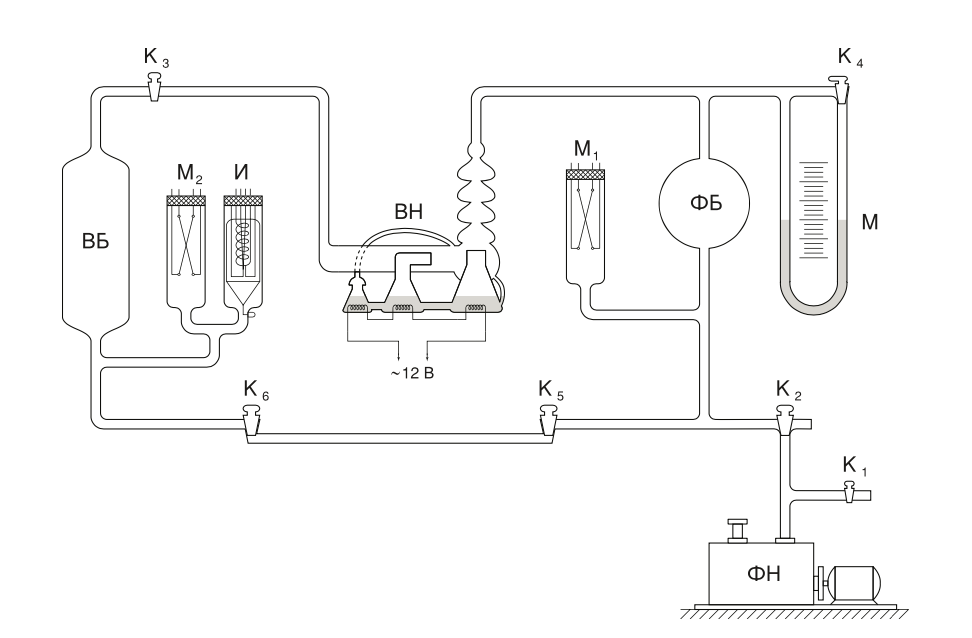
\includegraphics[scale = 0.75]{images/dr1.png}
  \caption{Схема экспериментальной установки}
  \label{fig:dr1}
\end{figure}

Установка изготовлена из стекла и состоит из: \\ 
— форвакуумного баллона (ФБ), \\ 
— высоковакуумного диффузионного насоса (ВН), \\ 
— высоковакуумного баллона (ВБ), \\ 
— масляного (М) и ионизационного (И) манометров, \\ 
— термопарных манометров (М1 и M2), \\ 
— форвакуумного насоса (ФН), \\ 
— соединительных кранов К1, К2, ..., К6. 

Кроме того, в состав установки входят: \\ 
— вариатор (автотрансформатор с регулируемым выходным напряжением) или реостат, \\ 
— амперметр для регулирования тока нагревателя диффузионного насоса.

\subsection*{Краны}

Все краны вакуумной установки — стеклянные.

Для герметизации используется вакуумная смазка. 

Если на поверхности шлифа видны круговые полосы, то кран либо плохо притёрт, либо неправильно смазан и может пропускать воздух. 

Краны работают лишь в том случае, если давление внутри крана меньше атмосферного. При этом пробка вдавливается внутрь крана.

\subsection*{Форвакуумный насос} 

Устройство и принцип действия ротационного пластинчатого форвакуумного насоса схематически показаны на рис. (\ref{fig:pre-vacuum_pump}).

\begin{figure}[h]
  \centering
  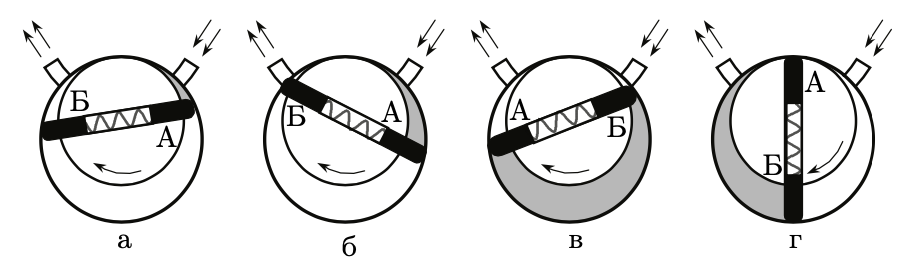
\includegraphics[scale = 0.75]{pre-vacuum_pump.png}
  \caption{\centering Схема действия ротационного двухпластинчатого форвакуумного насоса. В положениях «а» и «б» пластина «А» засасывает разреженный воздух из откачиваемого объёма, а пластина «Б» вытесняет ранее захваченный воздух в атмосферу. В положениях «в» и «г» пластины поменялись ролями}
  \label{fig:pre-vacuum_pump}
\end{figure}

В цилиндрической полости массивного корпуса размещен эксцентрично ротор так, что он постоянно соприкасается своей верхней частью с корпусом. В диаметральный разрез ротора вставлены две пластины, раздвигаемые пружиной и плотно прижимаемые к поверхности полости.

Они разделяют объём между ротором и корпусом на две части. Действие насоса ясно из изображённых на рис. (\ref{fig:pre-vacuum_pump}) последовательных положений пластин при вращении ротора по часовой стрелке. 

При работе с насосом следует помнить, что после остановки насоса в него обязательно нужно впускать воздух. Если этого не делать, то атмосферное давление может выдавить масло из насоса в патрубки и в вакуумную систему. Соединять насос с атмосферой следует при помощи кранов $K1$ или $K2$.

После включения насоса его присоединяют к установке не сразу, а через некоторое время, когда насос откачает собственный объём и пространство, расположенное до крана К2. Об этом можно судить по звуку насоса. Вначале насос сильно шумит, затем его звук делается мягким, и, наконец, в насосе возникает сухой стук, — это происходит, когда достигается хорошее разрежение.

\subsection*{Диффузионный насос}

Откачивающее действие диффузионного насоса основано на диффузии (внедрении) молекул разреженного воздуха в струю паров масла. 

Попавшие в струю молекулы газа увлекаются ею и уже не возвращаются назад. На прежнем их месте образуется пустота, которая немедленно заполняется следующими порциями газа, увеличивая степень разрежения газа в окрестности струи и оказывая таким образом сильное откачивающее воздействие на весь газ в откачиваемом объёме. 

Скорость откачки диффузионных насосов в сотни и тысячи раз превосходит скорость откачки форвакуумного насоса.

Устройство одной ступени масляного диффузионного насоса схематически показано на рис. (\ref{fig:diffusion_pump}).

\begin{figure}[h]
  \centering
  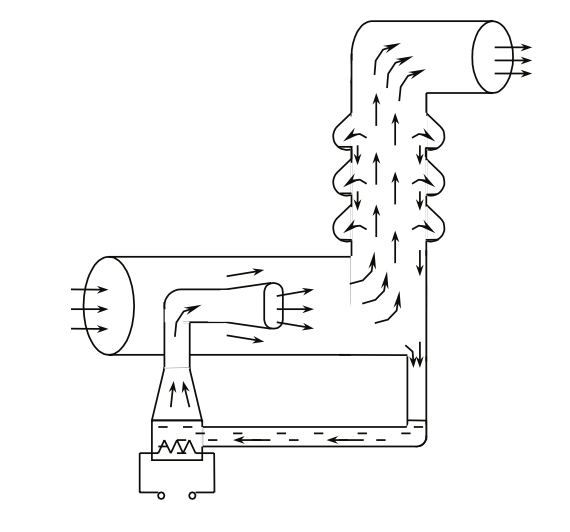
\includegraphics[scale = 0.75]{diffusion_pump.png}
  \caption{Схема работы диффузионного насоса}
  \label{fig:diffusion_pump}
\end{figure}

Масло, налитое в сосуд А, подогревается электрической печкой. Пары масла поднимаются по трубе Б и вырываются из сопла В. Струя паров увлекает молекулы газа, которые поступают из откачиваемого сосуда через трубку ВВ. Дальше смесь попадает в вертикальную трубу Г. Здесь масло осаждается на стенках трубы и маслосборников и стекает вниз, а оставшийся газ через трубу ФВ откачивается форвакуумным насосом. 

Диффузионный насос работает наиболее эффективно при давлении, когда длина свободного прбега молекул воздуха примерно равна ширине кольцевого зазора между соплом В и стенками трубы ВВ. 

Если диффузионный насос включить при давлении, сравнимом с давлением насыщенного пара масла, то последнее никакой струи не создаст и масло будет просто окисляться и угорать.

Граничное давление, выше которого диффузионный насос включать нельзя, на вакуумметрах термопарных ламп отмечено красной линией ($\sim 1,2$ мВ).

\medskip 

Диффузионный насос, используемый в нашей установке (рис. 1), имеет две ступени и соответственно два сопла. Одно сопло вертикальное (первая ступень), второе сопло горизонтальное (вторая ступень). 

За второй ступенью имеется ещё одна печь, она осуществляет фракционирование масла. Легколетучие фракции масла, испаряясь, поступают в первую ступень. По этой причине плотность струи первой ступени выше, и эта ступень начинает откачивать газ при более высоком давлении в форвакуумной части установки. Вторая ступень обогащается малолетучими фракциями. Плотность струи второй ступени меньше, но меньше и давление насыщенных паров масла в этой ступени. 

Соответственно в откачиваемый объём поступает меньше паров масла, и его удаётся откачать до более высокого вакуума.

\medskip

При работе с диффузионным насосом необходимо придерживаться следующих правил:
\begin{itemize}
  \item Включать подогрев диффузионного насоса можно лишь после того, как вакуум в системе доведен до $5 \cdot 10^{-2}$ торр при помощи форвакуумного насоса. При недостаточном предварительном разрежении масло в диффузионном насосе портится.
  \item Не следует допускать слишком интенсивного кипения масла.
\end{itemize}

\subsection*{Масляный манометр}

\subsection*{Термопарный манометр}

\subsection*{Ионизационный манометр}

\subsection*{Процесс откачки}

\subsection*{Течение газа через трубу}

\section*{Ход эксперимента}

\begin{center}
  \textsf{I. Определение объёма форвакуумной и высоковакуумной частей установки}
\end{center}

\begin{enumerate}
  % Подготовим установку к работе. Запустим туда атмосферный воздух 
  \item Проверим, что кран К4 открыт. Откройте все краны, кроме К1 и К2.
  \item Впустите в установку атмосферный воздух через краны К1 и К2.
  \item Закройте краны К5 и К6 (поверните рукоятки кранов вверх), в этих кранах и соединяющем их капилляре «запирается» 50 см3 воздуха при атмосферном давлении (точный объём указан на установках).
  \item Закройте краны К1 и К2, включите форвакуумный насос и дайте ему откачать себя. Подключите установку к форвакуумному насосу краном К2 и откачайте установку до давления $10^{-2}$ торр. Давление измеряйте вакуумметром ВТ-2, соединённым с лампой М1.
  \item Повернув рукоятку крана К2, отсоедините установку от форвакуумного насоса. Выключите форвакуумный насос и откройте кран К1.
  \item Перекрыв кран К3, отделите высоковакуумную часть установки от форвакуумной.
  \item Закрыв кран К4, приведите в готовность масляный манометр.
  \item Откройте кран К5. «Запертый» воздух распространится по всему объёму форвакуумной части установки и повысит в ней давление. Измерьте это давление масляным манометром.
  \item Зная объём "запертого" воздуха (см. п. 3), найдите, пользуясь законом Бойля–Мариотта, объём $V_{\text{фв}}$ форвакуумной части.
  \item Откройте кран К3, чтобы газ, занимавший до сих пор только форвакуумную часть установки, заполнил и её высоковакуумную часть. Вновь измерьте показания манометра. Рассчитайте полный объём установки и объём высоковакуумной её части Vвв.
  \item Откройте кран К4.
  \item Измерения по пп. $1-10$ повторите ещё раз.

\begin{center}
  \textsf{II. Получение высокого вакуума и измерение скорости откачки}
\end{center}

\item Откачайте установку форвакуумным насосом. Убедитесь в том, что краны в установке повёрнуты так, что в ней не осталось "запертых" объёмов.
\item Если термопарные вакуумметры выключены, включите их и не выключайте до конца работы. Установите токи в лампах по их паспортам (токи должны быть указаны на приборах вакуумметров). Переключите прибор манометра в режим измерения ЭДС, определите величину термоэдс и по графику — давление в системе.
В некоторых термовакуумметрах ЭДС термопары и соответствую- щее ей давление указаны на шкале прибора.
\item После того как давление упадёт ниже $3 \cdot 10^{-2}$ торр, закройте кран К6 и начните высоковакуумную откачку. Для этого включите нагреватель диффузионного насоса и подождите около 10 минут. Убедитесь в том, что масло в насосе закипело и у края отверстия образовалась плёнка выбрасываемого из сопла и конденсирующегося на стенках масла. При работе диффузионного насоса должен работать и форвакуумный насос.
Манометр M1 должен показывать давление около $10^{-2}$ торр, а показания милливольтметра манометра М2 должны быстро возрастать. В правильно отградуированном манометре стрелка должна дойти до конца шкалы.
\item Включите ионизационный манометр. Порядок его включения указан в инструкции на столе установки.
\item Измерьте предельное давление Pпр в системе и запишите его. При P < 10−4 торр убедитесь в правильности градуировки термоманометра М2. При необходимости сообщите преподавателю о том, что надо сде- лать поправку в паспорте.
\item Найдите скорость откачки по улучшению вакуума во время откачки. Для этого:
а) отключите откачку высоковакуумного баллона краном К3 и подо- ждите, пока вакуум достаточно ухудшится — до (5–9)·10−4 торр;
б) откройте кран К3 и отмечайте изменение показаний ионизацион- ного манометра во времени;
в) изобразите полученные результаты на графике, выбрав его коор- динаты так, чтобы было удобно сравнить их с формулой (4), то есть чтобы график имел вид прямой линии;
г) рассчитайте W системы.
\item Оцените величину потока Qн. Для этого:
а) перекройте кран К3 и прекратите таким образом откачку высоко- вакуумной части системы. При помощи ионизационного вакуумметра и секундомера следите за тем (и запишите в тетрадь), как ухудшается ва- куум. Опыт следует прекратить, когда давление в системе дорастет до (9–10)·10−4 торр. В этот момент кран К3 нужно снова открыть, чтобы не пережечь ионизационный манометр;
б) используя значение W, найденное в п. 18, и учтя, что уравнение (1) для этого случая принимает вид VввdP = (Qд + Qи)dt, оцените Qн.

\item Проведите повторные измерения по пунктам 18 и 19. Оцените пропуск- ную способность трубки от высоковакуумного баллона до насоса и срав- ните её с измеренной скоростью откачки.
\item Откройте кран К6 и введите таким образом в прибор искусственную течь (высоковакуумная часть установки соединена через капилляр с форвакуумной). Вакуум в установке должен ухудшиться. Измерьте установившееся давление Pуст и давление со стороны форвакуумной ча- сти капилляра.
\item Рассчитайте производительность насоса по различию Pуст и Pпр. Для этого найдите количество газа, протекающего через капилляр, по фор- муле (6). Запишем формулу (2) для случаев, когда капилляр перекрыт и когда он открыт:
PпрW = Q1, PустW = Q1 + d(PV )капилл . dt
В этих формулах символом Q1 обозначена сумма всех натеканий, кроме натекания через искусственную течь. Исключите из этих формул на- текание Q1 и найдите скорость откачки системы (в том сечении, где присоединен манометр).
Сравните получившееся значение W с полученным в п. 18. Проком- ментируйте причины возможного их несовпадения.
\item Выключите установку. Для этого:
а) выключите накал ионизационного манометра тумблером «Накал»
и дайте его лампе остыть, подождав 1–2 мин. Извлеките предохранитель и сдайте его преподавателю или лаборанту;
б) выключите подогрев диффузионного насоса, подождите, пока мас- ло в диффузионном насосе остынет (∼10 минут);
в) краном К2 отсоедините установку от форвакуумного насоса, не сообщая её с атмосферой;
г) в этих условиях давление во всех частях установки должно быть одинаково, одинаковы должны быть и показания термопарных мано- метров M1 и М2. Если они различаются, то отрегулируйте манометр М1 по показаниям термовакуумметра М2, уже откалиброванного при высоком вакууме;
д) выключите форвакуумный насос и, когда он остановится, соеди- ните его с атмосферой краном К1, не напуская атмосферу в установку;
е) выключите вакуумметры тумблерами «Сеть».

\end{enumerate}

\section*{Обработка результатов измерений}

\begin{table}[h]
  \caption{}
  \begin{tabular}{|c|c|c|c|}
      \hline $h_1^{\text{фв}}$, мм  &  $h_2^{\text{фв}}$, мм & $\Delta h^{\text{фв}}$, мм  &  $V^{\text{фв}}$, см$^3$ \\
      \hline
      347 & 93  &   & 2215 \\
      350 & 96  &   & 2215 \\
      \hline 
  \end{tabular}
  \label{tab:}
\end{table}

\begin{table}[h]
  \caption{}
  \begin{tabular}{|c|c|c|c|р}
      \hline $h_1^{\text{фв}}$, мм  &  $h_2^{\text{фв}}$, мм & $\Delta h^{\text{фв}}$, мм  &  $V^{\text{фв}}$, см$^3$ \\
      \hline
      305 & 142 &   & 1265 \\
       &  &   &   \\
      \hline 
  \end{tabular}
  \label{tab:}
\end{table}

\section*{Вывод}
\end{document}
